\vspace{-3mm}

\section{Experiments}


\textbf{Experimental setup.} \label{sec:experimental_setup}
For language tasks, we use RoBERTa-large \cite{liu2019roberta} as the backbone model, while ViT-large \cite{dosovitskiy2020image} is used for image tasks. 
The LoRA rank is set to $r=8$, and the scaling factor is set to $\alpha=8$. 
We consider a federated setting with $K=6$ clients for language tasks and $K=3$ clients for the vision tasks, with full client participation in every communication round.
Data are partitioned using a Dirichlet distribution with $\alpha=0.5$, except for SQuAD \cite{rajpurkar2016squad, rajpurkar2018know}, where data are equally partitioned across clients.
Training is conducted for $T=100$ communication rounds, with $\tau=10$ local steps per round. 
Following the empirical setup of \cite{sun2024improving}, the learning rate $\eta$ is selected from $\{0.05, 0.1, 0.25\}$ for FedLoRA and from $\{0.1, 0.25, 0.5, 1.0\}$ for all other methods. 
The batch size is set to $B=128$. 
For DP-SGD, we set the target failure probability to $\delta = 10^{-5}$ and fix the clipping norm at $C=2$. 
The differential privacy budget $\epsilon$ is computed using Opacus 
\cite{yousefpour2021opacus}. All experiments were run on RTX Pro $6000$ GPUs. Additional details are provided in Appendix~\ref{app:experimental_detail}. Unless otherwise specified, all experiments follow the settings described 
in Section~\ref{sec:experimental_setup} and Appendix~\ref{app:experimental_detail}.


% To quantify the contribution of each LoRA component, our scoring function is derived from a second-order approximation of the loss, which incorporates curvature information via the Hessian. 
% While this formulation provides a principled criterion, directly computing the Hessian is computationally prohibitive in practice.

\begin{wraptable}{r}{0.38\linewidth}
\vspace{-12pt}
\centering
\scriptsize
\setlength{\tabcolsep}{5.5pt}
\renewcommand{\arraystretch}{1.15}
\newcommand{\std}[1]{\,{\tiny$\pm$}\,\tiny #1}
\caption{Comparison on MNLI under DP-SGD ($\epsilon = 3$).}
\label{tab:mnli_variant}
\begin{tabular}{lcc}
\toprule
\textbf{Method} & \textbf{MNLI (m)} & \textbf{MNLI (mm)} \\
\midrule
Proposed  (FD)       & 79.15\std{0.23} & 80.03\std{0.40} \\
Proposed (HVP)   & 80.29\std{0.84} & 81.29\std{0.80} \\
\bottomrule
\vspace{-20pt}
\end{tabular}
\end{wraptable} 
For the proposed AS-LoRA, the warm-up ratio is set to $0.1$.  The temperature parameters are set to $T^0 = 2.0$, $T_{\min} = 0.2$, and $\gamma = 0.95$. While the proposed scoring function provides a theoretically grounded criterion,
direct Hessian computation is computationally prohibitive at the scale of large
pretrained models. To make the curvature-aware score practical, we consider two
approximation strategies, Hessian-Vector Products (HVP) \cite{pearlmutter1994fast} and Finite-Difference (FD) \cite{nocedal2006numerical} estimation, which are described in Appendix \ref{sec:Appendix B}. As shown in Table~\ref{tab:mnli_variant}, HVP-based scoring
achieves better performance, whereas FD-based scoring yields competitive
results without explicitly forming or storing the Hessian matrix. We
adopt the FD-based criterion in all subsequent experiments, as it preserves the
curvature-aware nature of the proposed score while maintaining practical
computational cost.

\textbf{Baselines.} We compare our method with the following baselines, which directly align with the design objective of AS-LoRA. Methods that address only the aggregation error~\cite{wang2024flora, singhal2024fedex, bai2024federated} are excluded from comparison, as they have been shown to suffer significant performance degradation under DP noise~\cite{lee2025fedsvd}.\\
\phantom{a}\textbf{FedLoRA} \cite{zhang2024towards}: Both $A$ and $B$ are locally trained and independently aggregated at the server.\\
\phantom{a}\textbf{FFA-LoRA} \cite{sun2024improving}: $A$ is frozen, and only $B$ is locally trained and aggregated.\\
\phantom{a}\textbf{RoLoRA} \cite{chen2025robust}: In odd-numbered rounds, $A$ is frozen and only $B$ is locally trained and aggregated.\\\phantom{a}In even-numbered rounds, $B$ is frozen and only $A$ is locally trained and aggregated.

\begin{table*}[h]
\centering
\scriptsize
\setlength{\tabcolsep}{3pt}
\renewcommand{\arraystretch}{1.05}
\newcommand{\std}[1]{\,{\tiny$\pm$}\,\tiny #1}

\caption{Performance comparison on the GLUE benchmark \cite{wang2018glue} under different privacy budgets.}
\label{tab:glue_dp}

\resizebox{\textwidth}{!}{
\begin{tabular}{c l c c c c c c c}
\toprule
\textbf{DP Budget} & \textbf{Method} & \textbf{QNLI} & \textbf{MNLI (m)} & \textbf{MNLI (mm)} & \textbf{SST-2} & \textbf{QQP}  & \textbf{SNLI} & \textbf{AVG}\\
\midrule

\multirow{4}{*}{$\epsilon = 3$}
 & FedLoRA   & \underline{72.43}\std{10.56} & 63.76\std{8.24} & 64.98\std{8.65} & 91.37\std{1.63} & 67.86\std{10.47} & 78.19\std{2.04} & 73.10\std{10.36} \\
 & FFA-LoRA  & 68.18\std{11.72} & 65.06\std{5.40} & 67.51\std{5.34} & 91.00\std{0.98} & \underline{75.79}\std{1.28} & 77.91\std{7.49} & 74.24\std{8.70} \\
 & RoLoRA    & 65.02\std{13.32} & \underline{69.15}\std{4.50} & \underline{71.02}\std{3.93} & \underline{91.37}\std{0.63} & 72.86\std{1.21} & \underline{82.22}\std{1.49} & \underline{75.27}\std{8.36} \\
 & Proposed  & \textbf{81.06}\std{1.34} & \textbf{79.15}\std{0.23} & \textbf{80.03}\std{0.40} & \textbf{92.86}\std{0.44} & \textbf{78.51}\std{0.38} & \textbf{85.23}\std{0.77} & \textbf{82.81}\std{4.93} \\
\midrule

\multirow{4}{*}{$\epsilon = 1$}
 & FedLoRA   & 55.72\std{1.40} & 58.03\std{8.05} & 59.37\std{8.94} & 57.57\std{0.37} & 65.72\std{9.90} & 74.79\std{1.63} & 61.87\std{6.56} \\
 & FFA-LoRA  & \textbf{71.95}\std{7.92} & \underline{62.70}\std{7.67} & \underline{65.04}\std{7.72} & \underline{79.27}\std{11.71} & 71.00\std{2.41} & \underline{81.37}\std{1.57} & \underline{71.89}\std{6.56} \\
 & RoLoRA    & 53.85\std{5.34} & 59.91\std{10.66} & 61.37\std{10.73} & 62.99\std{13.43} & \underline{73.10}\std{1.59} & 80.97\std{0.79} & 65.37\std{9.26} \\
 & Proposed  & \underline{71.52}\std{12.50} & \textbf{76.71}\std{0.92} & \textbf{77.54}\std{0.77} & \textbf{80.76}\std{14.08} & \textbf{74.94}\std{1.78} & \textbf{84.32}\std{0.64} & \textbf{77.63}\std{4.10} \\
\bottomrule
\end{tabular}
}
\vspace{-16pt}
\end{table*}

% \begin{table*}[h]
% \centering
% \scriptsize
% \setlength{\tabcolsep}{2pt}
% \renewcommand{\arraystretch}{1.05}
% \newcommand{\std}[1]{\,{\tiny$\pm$}\,\tiny #1}

% \caption{Performance comparison on SQuAD benchmarks \cite{rajpurkar2016squad, rajpurkar2018know} under different privacy budgets.}
% \label{tab:squad_dp}

% \begin{tabular}{c l c c c c}
% \toprule
% \textbf{DP Budget} & \textbf{Method} & \textbf{SQuAD v1.1 (EM)} & \textbf{SQuAD v1.1 (F1)} & \textbf{SQuAD v2.0 (EM)} & \textbf{SQuAD v2.0 (F1)} \\
% \midrule

% \multirow{3}{*}{$\epsilon = 3$}
%  & FFA-LoRA  & \underline{73.65}\std{2.71} & $\mathbf{83.95}$\std{1.68} & \underline{57.22}\std{3.12} & \underline{61.26}\std{3.48} \\
%  & RoLoRA    & 70.75\std{1.85} & 81.45\std{1.83} & 53.42\std{1.17} & 56.70\std{1.10} \\
%  & Proposed  & $\mathbf{73.80}$\std{1.31} & \underline{83.91}\std{1.42} & $\mathbf{61.18}$\std{2.75} & $\mathbf{65.18}$\std{3.05} \\
% \midrule

% \multirow{3}{*}{$\epsilon = 1$}
%  & FFA-LoRA  & \underline{71.99}\std{2.35} & \underline{82.60}\std{1.83} & \underline{56.15}\std{1.45} & \underline{60.41}\std{2.00} \\
%  & RoLoRA    & 63.45\std{1.49} & 75.35\std{1.27} & 52.13\std{0.67} & 54.44\std{0.60} \\
%  & Proposed  & $\mathbf{72.66}$\std{1.82} & $\mathbf{83.05}$\std{1.62} & $\mathbf{58.54}$\std{2.37} & $\mathbf{62.34}$\std{2.87} \\
% \bottomrule
% \end{tabular}
% \end{table*}

% \begin{table*}[h]
% \centering
% \scriptsize
% \setlength{\tabcolsep}{2pt}
% \renewcommand{\arraystretch}{1.05}
% \newcommand{\std}[1]{\,{\tiny$\pm$}\,\tiny #1}

% \caption{Performance comparison on CIFAR-100 \cite{krizhevsky2009learning} and Tiny-imageNet \cite{deng2009imagenet} benchmarks under different privacy budgets.}
% \label{tab:vision_dp}

% \begin{tabular}{c l c c}
% \toprule
% \textbf{DP Budget} & \textbf{Method} & \textbf{CIFAR-100} & \textbf{Tiny-ImageNet} \\
% \midrule

% \multirow{3}{*}{$\epsilon = 3$}
%  & FFA-LoRA  & 87.23\std{0.17} & \underline{85.53}\std{0.08} \\
%  & RoLoRA    & \underline{87.50}\std{0.20} & 84.67\std{0.01} \\
%  & Proposed  & $\mathbf{89.57}$\std{0.20} & $\mathbf{86.72}$\std{0.11} \\
% \midrule

% \multirow{3}{*}{$\epsilon = 1$}
%  & FFA-LoRA  & \underline{84.74}\std{0.13} & \underline{83.62}\std{0.27} \\
%  & RoLoRA    & 84.50\std{0.27} & 82.24\std{0.05} \\
%  & Proposed  & $\mathbf{85.49}$\std{0.20} & $\mathbf{83.80}$\std{0.03} \\
% \bottomrule
% \end{tabular}
% \end{table*}
\begin{table*}[h]
\centering
\scriptsize
\setlength{\tabcolsep}{2pt}
\renewcommand{\arraystretch}{1.05}
\newcommand{\std}[1]{\,{\tiny$\pm$}\,\tiny #1}

\caption{Performance comparison on SQuAD benchmarks \cite{rajpurkar2016squad, rajpurkar2018know},CIFAR-100 \cite{krizhevsky2009learning} and Tiny-imageNet \cite{deng2009imagenet} under different privacy budgets.}
\label{tab:squad_vision_dp}
\begin{tabular}{c l cc cc cc}
\toprule
\textbf{DP Budget} & \textbf{Method} 
& \multicolumn{4}{c}{\textbf{Question Answering}} 
& \multicolumn{2}{c}{\textbf{Image Classification}} \\

\cmidrule(lr){3-6} \cmidrule(lr){7-8}
& 
& \textbf{SQuAD v1.1 (EM)} & \textbf{SQuAD v1.1 (F1)} 
& \textbf{SQuAD v2.0 (EM)} & \textbf{SQuAD v2.0 (F1)} 
& \textbf{CIFAR-100} & \textbf{Tiny-ImageNet} \\

\midrule

\multirow{3}{*}{$\epsilon = 3$}
& FFA-LoRA  
& \underline{72.30}\std{3.52} & \underline{82.83}\std{2.83} 
& \underline{55.90}\std{3.66} & \underline{59.92}\std{3.93} 
& 87.37\std{0.26} & \underline{85.50}\std{0.15} \\

& RoLoRA    
& 69.75\std{2.70} & 80.63\std{2.30} 
& 53.58\std{1.22} & 56.88\std{1.16} 
& \underline{87.75}\std{0.40} & 84.62\std{0.13} \\

& Proposed  
& $\textbf{73.98}$\std{1.36} & $\textbf{83.99}$\std{1.17} 
& $\textbf{60.59}$\std{2.97} & $\textbf{64.23}$\std{3.62} 
& $\textbf{89.55}$\std{0.20} & $\textbf{86.66}$\std{0.32} \\

\midrule

\multirow{3}{*}{$\epsilon = 1$}
& FFA-LoRA  
& \underline{70.42}\std{3.91} & \underline{81.24}\std{3.26} 
& \underline{54.33}\std{3.91} & \underline{58.58}\std{4.16} 
& \underline{84.79}\std{0.23} & \underline{83.52}\std{0.26} \\

& RoLoRA    
& 61.69\std{3.81} & 73.94\std{3.10} 
& 51.48\std{1.47} & 53.59\std{1.80} 
& 84.64\std{0.38} & 82.34\std{0.14} \\

& Proposed  
& $\textbf{72.78}$\std{1.50} & $\textbf{83.23}$\std{1.37} 
& $\textbf{58.09}$\std{2.57} & $\textbf{61.64}$\std{3.16} 
& $\textbf{85.62}$\std{0.24} & $\textbf{83.71}$\std{0.13} \\

\bottomrule
\end{tabular}
\vspace{-0pt}
\end{table*}
% \begin{table*}[h]
% \centering
% \scriptsize
% \setlength{\tabcolsep}{2pt}
% \renewcommand{\arraystretch}{1.05}
% \newcommand{\std}[1]{\,{\tiny$\pm$}\,\tiny #1}

% \caption{Performance comparison on SQuAD benchmarks \cite{rajpurkar2016squad, rajpurkar2018know},CIFAR-100 \cite{krizhevsky2009learning} and Tiny-imageNet \cite{deng2009imagenet} under different privacy budgets.}
% \label{tab:squad_vision_dp}

% \begin{tabular}{c l cc cc cc}
% \toprule
% \textbf{DP Budget} & \textbf{Method} 
% & \multicolumn{4}{c}{\textbf{Question Answering}} 
% & \multicolumn{2}{c}{\textbf{Image Classification}} \\

% \cmidrule(lr){3-6} \cmidrule(lr){7-8}
% & 
% & \textbf{SQuAD v1.1 (EM)} & \textbf{SQuAD v1.1 (F1)} 
% & \textbf{SQuAD v2.0 (EM)} & \textbf{SQuAD v2.0 (F1)} 
% & \textbf{CIFAR-100} & \textbf{Tiny-ImageNet} \\

% \midrule

% \multirow{3}{*}{$\epsilon = 3$}
% & FFA-LoRA  
% & \underline{73.65}\std{2.71} & $\mathbf{83.95}$\std{1.68} 
% & \underline{57.22}\std{3.12} & \underline{61.26}\std{3.48} 
% & 87.23\std{0.17} & \underline{85.53}\std{0.08} \\

% & RoLoRA    
% & 70.75\std{1.85} & 81.45\std{1.83} 
% & 53.42\std{1.17} & 56.70\std{1.10} 
% & \underline{87.50}\std{0.20} & 84.67\std{0.01} \\

% & Proposed  
% & $\mathbf{73.80}$\std{1.31} & \underline{83.91}\std{1.42} 
% & $\mathbf{61.18}$\std{2.75} & $\mathbf{65.18}$\std{3.05} 
% & $\mathbf{89.57}$\std{0.20} & $\mathbf{86.72}$\std{0.11} \\

% \midrule

% \multirow{3}{*}{$\epsilon = 1$}
% & FFA-LoRA  
% & \underline{71.99}\std{2.35} & \underline{82.60}\std{1.83} 
% & \underline{56.15}\std{1.45} & \underline{60.41}\std{2.00} 
% & \underline{84.74}\std{0.13} & \underline{83.62}\std{0.27} \\

% & RoLoRA    
% & 63.45\std{1.49} & 75.35\std{1.27} 
% & 52.13\std{0.67} & 54.44\std{0.60} 
% & 84.50\std{0.27} & 82.24\std{0.05} \\

% & Proposed  
% & $\mathbf{72.66}$\std{1.82} & $\mathbf{83.05}$\std{1.62} 
% & $\mathbf{58.54}$\std{2.37} & $\mathbf{62.34}$\std{2.87} 
% & $\mathbf{85.49}$\std{0.20} & $\mathbf{83.80}$\std{0.03} \\

% \bottomrule
% \end{tabular}
% \end{table*}

% \subsection{Ablation Study} 
% In this section, we perform ablation studies on the key components of the proposed method, including mode selection scopes, mode selection strategy, random projection, and score aggregation method.



\textbf{Comparison results.} All results are reported as mean $\pm$ standard deviation over $4$ runs with different seeds. Best results are shown in \textbf{bold} and second-best results are \underline{underlined}. Table~\ref{tab:glue_dp} reports the performance on the GLUE benchmark \cite{wang2018glue} under different privacy budgets. The proposed method consistently outperforms all baselines across tasks.
Under a privacy budget of $\epsilon = 3$, AS-LoRA achieves the best average score of $\mathbf{82.81}$, outperforming RoLoRA ($75.27$) by +$\mathbf{7.54}$ percentage points (pp). 
% Notable gains include +4.58 pp on MNLI (m), +7.97 pp on MNLI (mm), and +3.09 pp on SST-2.
Under a budget of $\epsilon = 1$, where training instability is more severe, AS-LoRA attains $\mathbf{77.64}$, surpassing FFA-LoRA ($\mathbf{71.89}$) by +$\mathbf{5.74}$ pp. In particular, significant improvements are observed on MNLI (mm) (+$12.50$ pp over FFA-LoRA) and consistent gains across SNLI and QQP.
As shown in Table~\ref{tab:squad_vision_dp}, these improvements extend beyond classification tasks. On SQuAD, AS-LoRA achieves higher performance across both v1.1 and v2.0 metrics, e.g., +$1.35$ EM and +$1.96$ F1 over FFA-LoRA on SQuAD v1.1 under $\epsilon = 3$. Moreover, the method consistently improves vision benchmarks, achieving +$2.34$ pp on CIFAR-100 and +$1.19$ pp on Tiny-ImageNet. Extended results on LoRA rank and heterogeneity of data distribution can be found in Appendix~\ref{app:alpha_rank}.


\begin{wraptable}{r}{0.52\linewidth}
\vspace{-13pt}
\centering
\scriptsize
\setlength{\tabcolsep}{2pt}
\renewcommand{\arraystretch}{1.05}
\newcommand{\std}[1]{\,{\tiny$\pm$}\,\tiny #1}

\caption{Comparison across mode selection granularity.(\textit{Per-client}: layer-wise and client-wise, \textit{AS-LoRA}: layer-wise and client-tied, \textit{Global}: layer-tied and client-tied)}
\label{tab:mode_granularity}

\begin{tabular}{c l c c c}
\toprule
\textbf{DP Budget} & \textbf{Method} & \textbf{MNLI (m)} & \textbf{MNLI (mm)} & \textbf{QQP} \\
\midrule

\multirow{3}{*}{$\epsilon$ = 3}
& Per-client & 72.73\std{2.07} & 73.73\std{2.23} & 63.18\std{0.00} \\
& AS-LoRA (ours) & $\textbf{79.15}$\std{0.23} & $\textbf{80.03}$\std{0.40} & $\textbf{78.51}$\std{0.38} \\
& Global & 75.74\std{2.53} & 76.98\std{2.44} & 73.61\std{2.75} \\

\midrule

\multirow{3}{*}{$\epsilon$ = 1}
& Per-client & 34.60\std{1.72} & 34.53\std{1.37} & 63.18\std{0.00} \\
& AS-LoRA (ours) & $\textbf{76.71}$\std{0.92} & $\textbf{77.54}$\std{0.77} & $\textbf{74.94}$\std{1.78} \\
& Global & 72.54\std{3.85} & 73.79\std{3.87} & 72.62\std{3.26} \\
\bottomrule
\end{tabular}
\vspace{-15pt}
\end{wraptable}

\textbf{Granularity of mode selection scope.}
While AS-LoRA performs layer-wise mode selection that is shared across all clients, we evaluate two alternatives to justify this design choice. Both are round-wise adaptive as AS-LoRA, but differ in selection granularity. \textit{Global} shares a single mode across all layers and clients, whereas \textit{Per-client} selects modes independently for each layer \emph{and} each client. As shown in Table~\ref{tab:mode_granularity}, \textit{Per-client}, yields the worst performance across all tasks and privacy budgets. It is because the aggregated model suffers from aggregation error. \textit{Global} also underperforms AS-LoRA. Sharing a single mode across all layers prevents the model from exploiting layer-specific dynamics. AS-LoRA strikes the right balance, reserving model expressiveness without compromising aggregation stability.


% \begin{table}[h]
% \centering
% \scriptsize
% \setlength{\tabcolsep}{2pt}
% \renewcommand{\arraystretch}{1.05}
% \newcommand{\std}[1]{\,{\tiny$\pm$}\,\tiny #1}

% \caption{Comparison across mode selection scopes.}
% \label{tab:mode_scope}

% \begin{tabular}{c l c c c}
% \toprule
% \textbf{DP Budget} & \textbf{Method} & \textbf{MNLI (m)} & \textbf{MNLI (mm)} & \textbf{QQP} \\
% \midrule

% \multirow{3}{*}{$\epsilon$ = 3}
% & Proposed (layer, client) & 73.32\std{1.68} & 74.46\std{1.64} & 63.18\std{0.00} \\
% & Proposed (layer) -- ours & $\mathbf{79.23}$\std{0.19} & $\mathbf{80.18}$\std{0.36} & $\mathbf{78.55}$\std{0.42} \\
% & Proposed & 76.20\std{2.89} & 77.32\std{2.87} & 73.77\std{3.35} \\

% \midrule

% \multirow{3}{*}{$\epsilon$ = 1}
% & Proposed (layer, client) & 34.32\std{1.62} & 34.31\std{1.29} & 63.18\std{0.00} \\
% & Proposed (layer) -- ours & $\mathbf{77.17}$\std{0.52} & $\mathbf{77.94}$\std{0.45} & $\mathbf{74.67}$\std{1.77} \\
% & Proposed & 72.78\std{4.68} & 74.14\std{4.67} & 73.00\std{3.82} \\

% \bottomrule
% \end{tabular}
% \end{table}

% \subsection{Analysis}
% In this section, we provide further analysis of the proposed method, including the effects of LoRA rank and data heterogeneity, smoothing kernel application, and comparison with an SVD-based method.



\begin{wraptable}{r}{0.49\linewidth}
\vspace{-13pt}
\centering
\scriptsize
\setlength{\tabcolsep}{2pt}
\renewcommand{\arraystretch}{1.05}
\newcommand{\std}[1]{\,{\tiny$\pm$}\,\tiny #1}

\caption{Comparison with FedSVD \cite{lee2025fedsvd} in performance and aggregation time.}
\label{tab:analysis_svd}

\begin{tabular}{c l c c c}
\toprule
\textbf{DP Budget} & \textbf{Method} & \textbf{Time (s)} & \textbf{MNLI (m)} & \textbf{MNLI (mm)} \\
\midrule

\multirow{4}{*}{$\epsilon = 3$}
& FedSVD(10) & 1.00 (33$\times$) & 78.16\std{1.01} & 79.43\std{1.21} \\
& FedSVD(5)  & 1.80 (60$\times$) & 77.06\std{1.47} & 79.07\std{1.10} \\
& FedSVD(1)  & 5.44 (181$\times$) & 78.49\std{0.89} & 79.75\std{0.68} \\
& Proposed   & \textbf{0.03 (1$\times$)} & \textbf{79.15}\std{0.23} & \textbf{80.03}\std{0.40} \\
\midrule

\multirow{4}{*}{$\epsilon = 1$}
& FedSVD(10) & 1.00 (33$\times$) & 74.24\std{1.48} & 75.69\std{1.45} \\
& FedSVD(5)  & 1.80 (60$\times$) & \textbf{76.97}\std{1.25} & \textbf{78.16}\std{1.13} \\
& FedSVD(1)  & 5.44 (181$\times$) & 76.62\std{0.77} & 77.79\std{0.60} \\
& Proposed   & \textbf{0.03 (1$\times$)} & 76.71\std{0.92} & 77.54\std{0.77} \\
\bottomrule
\end{tabular}

\vspace{-10pt}
\end{wraptable}

\textbf{Comparison with SVD-based method.} 
Table~\ref{tab:analysis_svd} compares AS-LoRA with \emph{FedSVD} \cite{lee2025fedsvd} the representative SVD-based method. FedSVD improves performance by introducing an additional SVD computation at the server. FedSVD$(n)$ applies SVD at every $n$-th communication rounds with standard FedAvg used otherwise.
Under $\epsilon=3$, the proposed method achieves the best performance while requiring substantially lower aggregation time. Under $\epsilon=1$, FedSVD$(5)$ shows slightly higher performance, but the gap is marginal. 
Moreover, while the proposed method relies on the FD-based score, it can scale to heavier approximations (HVP) as shown in Table~\ref{tab:mnli_variant}.




\begin{figure*}[h]
    \centering
    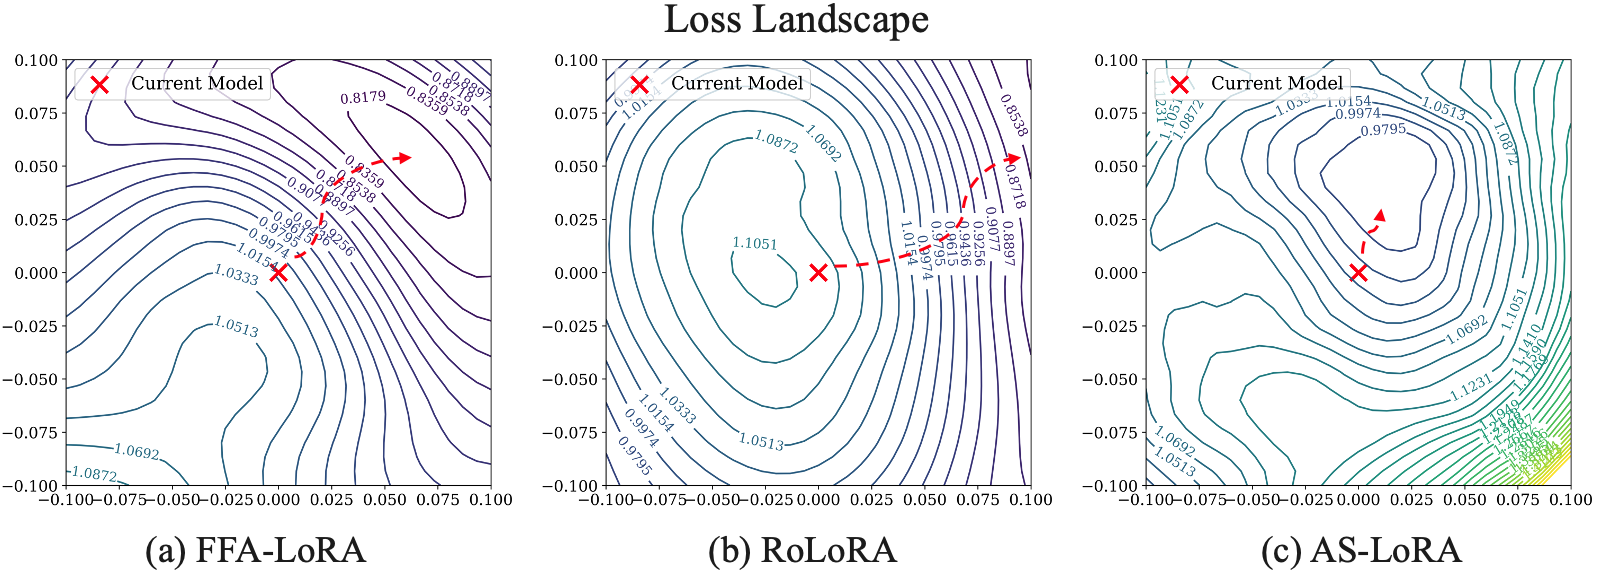
\includegraphics[width=1.0\textwidth]{figures/6_experiments/loss_landscape.png}
    \caption{Loss landscape visualization of FFA-LoRA, RoLoRA, and AS-LoRA trained on MNLI with $T=100$ and $\tau=10$ under DP-SGD ($\epsilon=3$).}
    \label{fig:loss_landscape}
    \vspace{-5pt}
\end{figure*}


\begin{wraptable}{r}{0.35\linewidth}
\vspace{-13pt}
\centering
\scriptsize
\setlength{\tabcolsep}{2pt}
\renewcommand{\arraystretch}{1.05}
\newcommand{\std}[1]{\,{\tiny$\pm$}\,\tiny #1}

\caption{Comparison of SAM-style perturbation sharpness on MNLI.} 
\label{tab:perturbation_sharpness}

\begin{tabular}{lcc}
\toprule
\textbf{Method} & \textbf{PS} & $\boldsymbol{\Delta}$\textbf{Acc} \\
\midrule
FFA-LoRA & 0.03608 \std{0.04565} & 0.981\std{1.182} \\
RoLoRA   & 0.01972 \std{0.02530} & 0.321\std{0.045} \\
AS-LoRA  & $\textbf{0.00992}$\std{0.01281} & $\textbf{0.247}$\std{0.282} \\
\bottomrule
\end{tabular}
\vspace{-5pt}
\end{wraptable}


\textbf{Sharpness and loss landscape analysis.} 
To empirically validate Theorem~\ref{thm:implicit}, which establishes that AS-LoRA's curvature-penalty score implicitly biases the trajectory toward flatter regions of the loss landscape, we measure the SAM-style perturbation sharpness
$
PS = L(w+\rho \hat g)-L(w), ~ 
\hat g = \nabla L(w)/\|\nabla L(w)\|,
$
together with the induced accuracy drop ($\Delta$Acc) \cite{foret2021sam}. The results in Table~\ref{tab:perturbation_sharpness} indicates that the solution found by AS-LoRA is more robust to local perturbations and lies in a flatter region of the loss surface. This observation is further supported by the loss landscape visualization in Figure~\ref{fig:loss_landscape}. Compared with FFA-LoRA and RoLoRA, the contour around the AS-LoRA solution appears to suggest a flatter optimization geometry. Such flatness is known to correlate with improved stability and generalization \cite{kaddour2022flat}, which is consistent with the empirical results in TABLE \ref{tab:glue_dp} and TABLE \ref{tab:squad_vision_dp}.

\begin{wraptable}{r}{0.34\textwidth}
\vspace{-13pt}
\centering
\scriptsize
\setlength{\tabcolsep}{2pt}
\renewcommand{\arraystretch}{1.05}
\newcommand{\std}[1]{\,{\tiny$\pm$}\,\tiny #1}
\caption{
    Comparison of curvature computation schedules in AS-LoRA under DP-SGD ($\epsilon=3$).
}
\label{tab:score_computation}
\begin{tabular}{lcc}
\toprule
\textbf{Method} & \textbf{MNLI (m)} & \textbf{MNLI (mm)} \\
\midrule
\multicolumn{3}{l}{\textit{Periodic computation}} \\
($f{=}5$)   & 77.99\std{1.17} & 79.39\std{1.07} \\
($f{=}10$)  & 78.83\std{1.08} & 79.76\std{0.80} \\
\midrule
\multicolumn{3}{l}{\textit{Late-phase computation}} \\
($T^*{=}80$) & 78.91\std{1.11} & 79.87\std{0.95} \\
($T^*{=}90$) & 78.85\std{0.88} & \textbf{80.11}\std{0.74} \\
\midrule
\multicolumn{3}{l}{\textit{Original}} \\
Proposed (ours) & \textbf{79.15}\std{0.23} & 80.03\std{0.40} \\
\bottomrule
\end{tabular}
\vspace{-20pt}
\end{wraptable}


\textbf{Overhead analysis.}
Under AS-LoRA with FD approximation, each client evaluates the local loss at two perturbed points 
$\mathcal{L}_k^t\!\left(W_t\pm \epsilon_{\mathrm{fd}} v_{a,k}^t(n)\right)$ per layer (Algorithm \ref{alg:score_fd}). In our setting, this incurs a $160\%$ increase in training cost over the baseline, which may be impractical for resource-constrained deployments. We therefore propose two complementary strategies that jointly reduce this overhead from $160\%$ to $\mathbf{8\%}$ while preserving the performance gains. \emph{One-sided FD.} Replacing the symmetric difference with the forward difference $\mathcal{L}_k^t\!\left(W_t+ \epsilon_{\mathrm{fd}} v_{a,k}^t(n)\right)- \mathcal{L}_k^t\!\left(W_t\right)$ requires only a single additional forward pass, halving the curvature-evaluation cost. \emph{Occasional curvature computation.} We reduce the frequency of computing the curvature part $g_a^\top H_a g_a$ in $S_a=\|g_a\|^2-\tfrac{\eta}{2}g_a^\top H_a g_a$, and uses only $\|g_a\|^2$, which is free through training, otherwise. We compare two scheduling variants: \emph{(i) Periodic computation}, inspired by the periodic SVD \cite{lee2025fedsvd}, evaluates the full score every $f \in \{5, 10\}$ rounds, and \emph{(ii) Late-phase computation} evaluates it only after round $T^* \in \{80, 90\}$. The latter is motivated by our empirical observation that $\|g_a\|^2$ dominate the optimization in early training, whereas $g_a^\top H_a g_a$ becomes informative as $\|g_a\|^2$ diminishes. As shown in Table~\ref{tab:score_computation}, late-phase computation matches the full FD-based AS-LoRA and incur only a marginal performance drop in terms of variance, causing only a $\mathbf{8\%}$ computation increase at $T^* = 90$ ($20\times$ reduction from the original). These results suggest that full per-round curvature scoring is unnecessary, and that selective computation, at the last phase in particular, can substantially reduce overhead. Communication overhead is negligible: AS-LoRA introduces only $N$ scalar scores (uplink) and $N$ mode bits (downlink) per round, accounting for less than $0.02\%$ of the active LoRA parameter traffic in our $24$-layer configuration. Detailed analyses are provided in Appendix~\ref{app:communication_overhead} and Appendix~\ref{app:computational_overhead}.

\textbf{Effect of gradient smoothing under DP-SGD.} 
Motivated by prior work~\cite{liu2026rethinking, liang2024differentially, wang2020dp} demonstrating that applying smoothing after Gaussian noise injection in DP-SGD improves utility, we investigate several smoothing strategies such as Gaussian, Laplacian, and EMA applied to our method. Detailed results are provided in Appendix~\ref{app:kernel}.

% AS-LoRA communicates one active component per layer, matching the communication cost of alternating methods ($P_B$ or $P_A$ per round).
% The only additional cost is $2N$ scalar scores (uplink) and $N$ mode bits (downlink) per round.
% For a 24-layer backbone, this amounts to $192$ bytes per client per round, less than $0.03\%$ of the active LoRA parameter traffic at hidden dimension 1024.

% To reduce the computational overhead of curvature-score computation, we consider two complementary strategies:
% \textbf{(i) one-sided FD} and \textbf{(ii) score computation strategies} (Periodic and Late-phase).
% Following the approximation in~\cite{kaplan2020scaling} 
% ($C_{\mathrm{bwd}} \approx 2C_{\mathrm{fwd}}$),
% the baseline training cost over $T{=}100$ rounds is
% $
% 3\tau T = 3{,}000\,C_{\mathrm{fwd}}.
% $
% Using one-sided FD, curvature scoring applied every $f{=}10$ rounds incurs
% $
% N_{\mathrm{target}} \cdot (T/f)
% = 48 \times 10
% = 480\,C_{\mathrm{fwd}},
% $
% which reduces the computational overhead by half compared to the
% central-difference scheme.
% We consider the following score computation strategies.:
% \textbf{(i) Periodic computation}, which computes curvature scores every
% $f \in \{5,10\}$ rounds and uses $\|\tilde{g}\|^2$ otherwise, and
% \textbf{(ii) Late-phase computation}, which applies $\|\tilde{g}\|^2$
% during the first $T^* \in \{80,90\}$ rounds and switches to curvature
% scoring afterward.

% As shown in Table~\ref{tab:score_computation}, Late-phase computation
% ($T^*{=}80$) incurs only a marginal performance drop of $-0.24$
% on MNLI (m) compared to the full proposed method.
% Moreover, Late-phase computation ($T^*{=}90$) even achieves higher
% MNLI (mm) performance than the full method by concentrating curvature
% scoring on the final 10 rounds.
% These results suggest that full per-round curvature scoring is unnecessary,
% and that selective computation can preserve most of the performance gains
% while substantially reducing the computational overhead. Detailed analyses are provided in Appendix~\ref{app:communication overhead} and Appendix~\ref{app:computational overhead}.
